\section{Hausdorffova míra a Hausdorffova dimenze}\label{sec:hausdorffova-mira-dimenze}

Způsobů,~jak definovat dimenzi je celá řada. Zatím jsme společně prozkoumali box-counting dimenzi (resp. některá její pojetí),~avšak lze najít více způsobů její definice\footnote{Některé další jsou sepsány např. v~\citep[str. 40]{Falconer2014}.}. Pravděpodobně však nejstarším exemplářem svého druhu je tzv. \emph{Hausdorffova dimenze} a s~ní související \emph{Hausdorffova míra},~které hrají ve fraktální geometrii velice podstatnou roli. Stále se však budeme zabývat pouze množinami v~$\R^n$. Jsou pojmenovány po německém matematikovi \name{Felixi Hausdorffovi} (1868--1942).
\begin{figure}[h]
    \centering
    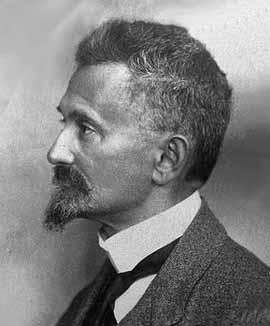
\includegraphics[width=0.4\textwidth]{felix-hausdorff.jpg}
    \caption[Felix Hausdorff,~1868--1942]{Felix Hausdorff\footnote{Převzato z~\cite{OConnorHausdorff2025}},~1868--1942}
    \label{fig:felix-hausdorff}
\end{figure}

\subsection{Definice Hausdorffovy míry}\label{subsec:hd-mira-definice}

\begin{definition}\label{def:hd-mira-delta}
    Nechť je dána množina $F\subseteq\R^n$ a $s>0$. Pak pro každé $\delta>0$ definujeme zobrazení
    \[\hausdorffdeltameasure{s}{\delta}(F)=\inf\set{\sum_{i=1}^{\infty}(\diam{F_i})^s\;\middle|\;F\subseteq\bigcup_{i=1}^\infty F_i\;,\;\diam{F_j}\leqslant\delta\;\text{pro}\;1\leqslant j\leqslant n}.\]
\end{definition}
Na první pohled si lze všimnout,~že pro $0<\delta_1<\delta_2$ je $\hausdorffdeltameasure{s}{\delta_1}(F)\leqslant\hausdorffdeltameasure{s}{\delta_2}(F)$. Jinými slovy,~pro $\delta\to 0$ hodnota $\hausdorffdeltameasure{s}{\delta}(F)$ klesá. Toto není nikterak těžké si rozmyslet,~neboť pro $\delta_1<\delta_2$ existuje $\delta_1$-pokrytí $\mathcal{F}_1$,~takové,~že je podpokrytím $\delta_2$-pokrytí $\mathcal{F}_2$ množiny $F$,~tedy $\mathcal{F}_1\subseteq\mathcal{F}_2$. To znamená,~že
\begin{align*}
    \hausdorffdeltameasure{s}{\delta_1}(F)&=\inf\set{\sum_{U\in\mathcal{F}_1}(\diam{U})^s\;\middle|\;\text{$\mathcal{F}_1$ je $\delta_1$-pokrytí}}\\
    &\leqslant\inf\set{\sum_{U\in\mathcal{F}_2}(\diam{U})^s\;\middle|\;\text{$\mathcal{F}_2$ je $\delta_2$-pokrytí}}=\hausdorffdeltameasure{s}{\delta_2}(F).
\end{align*}
Zároveň je z~definice \ref{def:hd-mira-delta} zjevné,~že $\mathcal{H}_\delta^s(F)\geqslant 0$.
\begin{definition}[Hausdorffova míra]\label{def:hausdorffova-mira}
    Nechť $F\subseteq\R^n$. Pak pro množinu $F$ definujeme \emph{$s$-dimenzionální Hausdorffovu míru}\index{míra!Hausdorffova} jako
    \[\hausdorffmeasure{s}(F)=\lim_{\delta\to 0}\hausdorffdeltameasure{s}{\delta}(F).\]
\end{definition}
Z přechodzího je zjevné, že limita v definici \ref{def:hausdorffova-mira} vždy existuje.

Bude dobré se přesvědčit, že je Hausdorffova míra mírou ve smyslu definice \ref{def:prostor-s-mirou}. Začneme však otázkou. \emph{Na jaké množině je potřeba Hausdorffovu míru $\hausdorffmeasure{s}$ uvažovat?} Odpověď nám poskytují tzv. \emph{borelovské množiny}\index{množina!borelovská}, které jsou pojmenovány po francouzském matematikovi \name{Émile Borelovi} (1871--1956).
\begin{figure}[h]
    \centering
    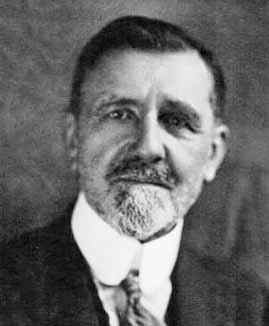
\includegraphics[width=0.4\textwidth]{Emile-Borel.jpeg}
    \caption[Émile Borel,~1871--1956]{Émile Borel\footnote{Převzato z \cite{OConnorBorel2025}},~1871--1956}
\end{figure}
Borelovské množiny hrají podstatnou roli v tzv. \emph{Deskriptivní teorii množin}. Nebudeme si zde vykládat všechny souvislosti, vystačíme si se základem. Takto nazýváme všechny množiny, které lze získat operacemi spočetného sjednocení a průniku otevřených množin z $X$. Označme systém takových množin jako $\mathcal{B}$. Na tomto základě pak definujeme tzv. \emph{$\sigma$-algebru borelovských množin na $X$}:
\[\borelsigmaalgebra(X)=\bigcap_{\substack{\mathcal{F}\supseteq\mathcal{B}\\\text{$\mathcal{F}$ je $\sigma$-algebra}}}\mathcal{F}.\]
Jinými slovy, $\borelsigmaalgebra(X)$ je nejmenší $\sigma$-algebra generovaná\footnote{Obecně $\sigma$-algebra $\mathcal{A}$ je generovaná množinou $X$, když
\[\mathcal{A}=\bigcap_{\substack{\mathcal{F}\supseteq X\\\text{$\mathcal{F}$ je $\sigma$-algebra}}}\mathcal{F}.\]
Tento fakt se někdy značí $\mathcal{A}=\sigma(X)$.} všemi otevřenými množinami z $X$.

Nás speciálně bude zajímat $\sigma$-algebra $\borelsigmaalgebra(\R^n)$.
\begin{lemma}[$\sigma$-subaditivita Hausdorffovy míry]\label{lem:Hausdorffova-mira-subaditivita}
    Nechť jsou dány množiny $A_1,A_2,\ldots$, kde $A_i\subseteq\R^n$ pro každé $i\in\N$. Pak pro každé $s\geqslant 0$ platí
    \[\hausdorffmeasure{s}\left(\bigcup_{i=1}^\infty A_i\right)\leqslant\sum_{i=1}^{\infty}\hausdorffmeasure{s}(A_i).\]
\end{lemma}
\begin{proof}
    Nechť $s\geqslant 0$. Pro každé $i\in\N$ a $\delta>0$ mějme pokrytí
    \[\mathcal{F}_i=\set{F_{i,1},F_{i,2},\dots}\]
    množiny $A_i$, takové, že pro každé $j\in\N$ a $\varepsilon$ platí
    \[\sum_{j=1}^{\infty}(\diam{F_{i,j}})^s\leqslant\hausdorffdeltameasure{s}{\delta}(A_i)+\dfrac{\varepsilon}{2^i}.\]
    Systém $\bigcup_{i=1}^\infty\mathcal{F}_i$ tedy tvoří $\delta$-pokrytí množiny $A=\bigcup_{i=1}^\infty A_i$. Celkově
    \begin{align*}
        \hausdorffdeltameasure{s}{\delta}\left(\bigcup_{i=1}^\infty A_i\right)&\leqslant\sum_{i,j\in\N}(\diam{F_{i,j}})^s=\sum_{i=1}^{\infty}\sum_{j=1}^{\infty}(\diam{F_{i,j}})^s\leqslant\sum_{i=1}^{\infty}\left(\hausdorffdeltameasure{s}{\delta}(A_i)+\dfrac{\varepsilon}{2^i}\right)\\
        &=\sum_{i=1}^{\infty}\hausdorffdeltameasure{s}{\delta}(A_i)+\varepsilon.
    \end{align*}
    Limitním přechodem $\delta\to 0$ a aplikací Leviho věty\footnote{\emph{Leviho věta o záměně pořadí limity a lebesgueova integrálu} říká, že je-li posloupnost nezáporných měřitelných funkcí $\set{f_n}_{n=1}^\infty$ neklesající, tj.
    \[f_1\leqslant f_2\leqslant\dots\]
    na prostoru $(X,\mathcal{A},\mu)$ a zároveň $\lim_{n\to\infty}f_n(x)=f(x)$ pro každé $x\in X$, pak
    \[\lim_{n\to\infty}\int_X f_n\dx[\mu]=\int_X \lim_{n\to\infty}f_n\dx[\mu].\]
    Zde je speciálně $\mu$ aritmetická míra $X=\N$, a $f_n(i)$ lze volit např. $\hausdorffdeltameasure{s}{1/n}(A_i)$. Z Heineho věty víme, že
    \[\lim_{n\to\infty}\hausdorffdeltameasure{s}{1/n}(A_i)=\lim_{\delta\to 0}\hausdorffdeltameasure{s}{\delta}(A_i)=\hausdorffmeasure{s}(A_i).\]
    }
    dostáváme
    \begin{align*}
        \hausdorffmeasure{s}\left(\bigcup_{i=1}^\infty A_i\right)&=\lim_{\delta\to 0}\hausdorffdeltameasure{s}{\delta}\left(\bigcup_{i=1}^\infty A_i\right)\leqslant\lim_{\delta\to 0}\sum_{i=1}^{\infty}\hausdorffdeltameasure{s}{\delta}(A_i)+\varepsilon=\sum_{i=1}^{\infty}\lim_{\delta\to 0}\hausdorffdeltameasure{s}{\delta}(A_i)+\varepsilon\\
        &=\sum_{i=1}^{\infty}\hausdorffmeasure{s}(A_i)+\varepsilon.
    \end{align*} 
\end{proof}
\begin{theorem}\label{thm:hausdorffova-mira-je-mira}
    $(\R^n,\borelsigmaalgebra(\R^n),\hausdorffmeasure{s})$ tvoří prostor s mírou.
\end{theorem}
Věta \ref{thm:hausdorffova-mira-je-mira} říká, že omezíme-li se na $\sigma$-agebru borelovských množin, pak $\hausdorffmeasure{s}$ je skutečně mírou.
\begin{proof}
    Fakt, že $\hausdorffmeasure{s}(\emptyset)=0$ je zjevný. Stačí zvolit pokrytí množinami s nulovým průměrem, tedy např. prázdnými množinami.
\end{proof}

\todo{Doplnit důkaz,~že Hausdorffova míra je mírou}